%\index{examples|see{data}}
%\index{graphs|see{plots}}\index{multicollinearity|see{collinearity}}

\setcounter{chapter}{9}
\chapter{Longitudinal and Panel Data Models}

{\small \textit{Chapter Preview}. Longitudinal data, also known as
panel data, are composed of a cross-section of subjects that we
observe repeatedly over time. Longitudinal data allow us to study
cross-sectional and dynamic patterns simultaneously; this chapter
describes several techniques for visualizing longitudinal data. Two
types of models are introduced, fixed and random effects models.
This chapter shows how to estimate fixed effects models using
categorical explanatory variables. Estimation for random effects
models is deferred to a later chapter; this chapter describes when
and how to use these models.}

\section{What are Longitudinal and Panel Data?}\label{S10:Intro}

In Chapters 1--6 we studied cross-sectional regression techniques
that allowed us to predict a dependent variable $y$ using
explanatory variables $x$. For many problems, the best predictor is
a value from the preceding period; the times series methods we
studied in Chapters 7--9 use the history of a dependent variable for
prediction. For example, an actuary seeking to predict insurance
claims for a small business will often find that last year's claims
are the best predictor. However, a limitation of time series methods
is that they are based on having available many observations over
time (typically 30 or more). When studying annual claims from a
business, a long time series is rarely available; either businesses
do not have the data or, if they do, it is unreasonable to use the
same stochastic model for today's claims as for those 30 years in
the past. We would like a model that allows us to use information
about company characteristics, explanatory variables such as
industry, number of employees, age and gender composition, and so
forth, as well as \emph{recent} claims history. That is, we need a
model that combines cross-sectional regression explanatory variables
with time series lagged dependent variables as predictors.

\emph{Longitudinal data} analysis represents a marriage of
regression and time series analysis. Longitudinal data are composed
of a cross-section of subjects that we observe repeatedly, over
time. Unlike regression data, with longitudinal data we observe
subjects over time. By observing a cross-section repeatedly,
analysts can make better assessments of regression relationships
with a longitudinal data design compared to a regression design.
Unlike time series data, with longitudinal data we observe many
subjects. By observing time series behavior over many subjects, we
can make informed assessments of temporal patterns even when only a
short (time) series is available.  Time patterns are also known as
\emph{dynamic}. With longitudinal data, we can study cross-sectional
and dynamic patterns simultaneously.

\marginparjed{With longitudinal data, we can study cross-sectional
and dynamic patterns simultaneously.}

The descriptor ``panel data'' comes from surveys of individuals. In
this context, a ``panel'' is a group of individuals surveyed
repeatedly over time. We use the terms ``longitudinal data'' and
``panel data'' interchangeably although, for simplicity, we often
use only the former term.

As we have seen in our Chapter 6 discussion of omitted variables,
any new variable can alter our impressions and models of the
relationship between $y$ and an $x$. This is also true of lagged
dependent variables. The following example demonstrates that the
introduction of a lagged dependent variable can dramatically impact
a cross-sectional regression relationship.\index{omitted variable}

\linejed\index{examples!divorce rates}

\textbf{Example: Divorce Rates.} \ecaptionjed{Divorce Rates} Figure
\ref{F10:Divorce} shows the 1965 divorce rates versus AFDC (Aid to
Families with Dependent Children) payments for the fifty states. For
this example, each state represents an observational unit, the
divorce rate is the dependent variable of interest and the level of
AFDC payment represents a variable that may contribute information
to our understanding of divorce rates.

\begin{figure}[htp]
  \begin{center}
    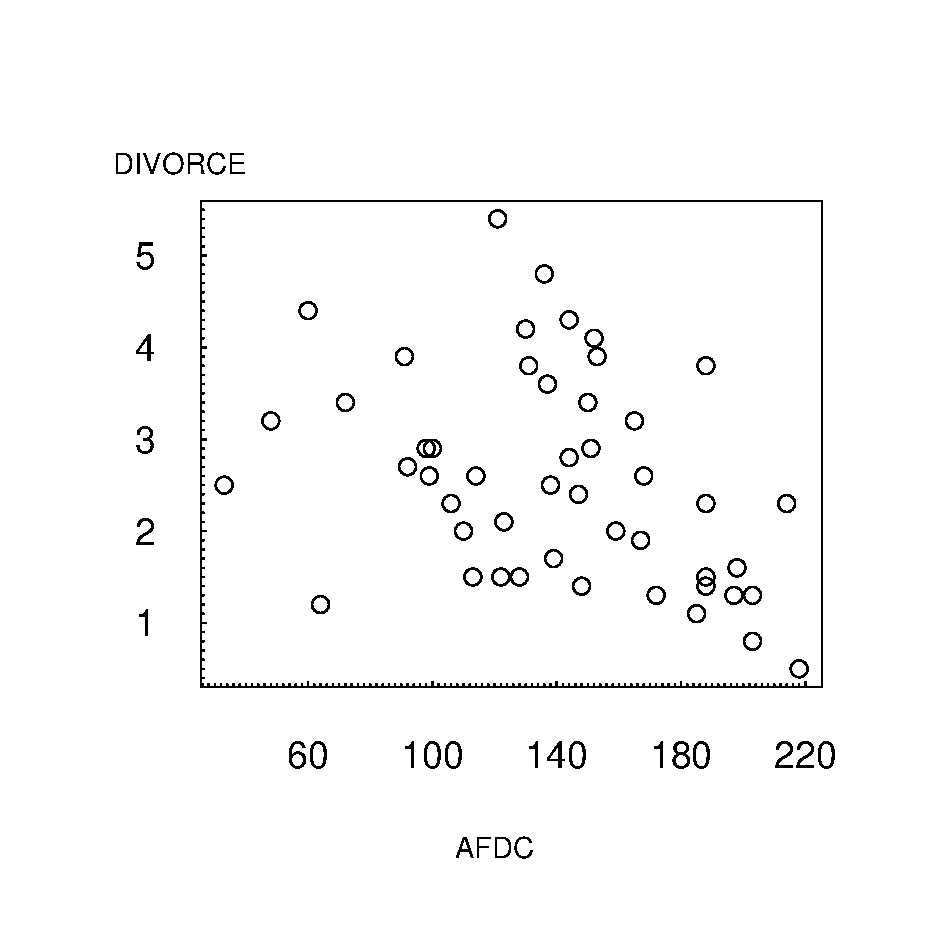
\includegraphics[width=0.45\textwidth]
        {Chapter10LongData/F10Divorce65.eps}
      \hfill
            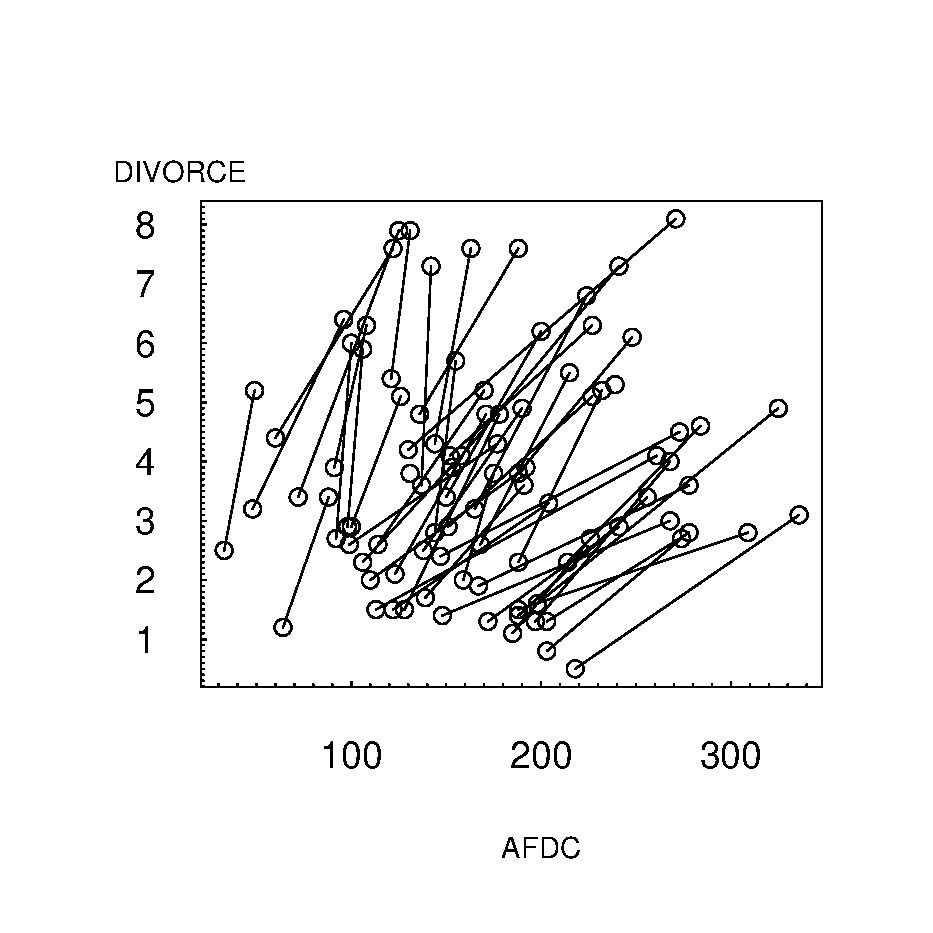
\includegraphics[width=0.45\textwidth]
       {Chapter10LongData/F10DivorcePanel.eps}
      \end{center}
           \parbox[t]{2.5in}{\caption {\label{F10:Divorce}
           {\small Plot of 1965 Divorce versus AFDC Payments.}}} \hfill
        \parbox[t]{2.5in}{\caption {\label{F10:Divorce2}
           {\small Plot of Divorce versus AFDC Payments - 1965 and
           1975.}}}
\end{figure}



Figure \ref{F10:Divorce} shows a negative relation; the
corresponding correlation coefficient is -0.37. Some argue that this
negative relation is counter-intuitive in that one would expect a
positive relation between welfare payments (AFDC) and divorce rates;
states with desirable cultural climates enjoy both low divorce rates
and low welfare payments. Others argue that this negative
relationship is intuitively plausible; wealthy states can afford
high welfare payments and produce economic and cultural climates
conducive to low divorce rates. Because the data are observational,
it is not appropriate to argue for a causal relationship between
welfare payments and divorce rates without additional economic or
sociological theory.

Another plot, not displayed here, shows a similar negative relation
for 1975; the corresponding correlation is -0.425.

Figure \ref{F10:Divorce2} shows both the 1965 and 1975 data; a line
connects the two observations within each state. The line represents
a change over time (dynamic), not a cross-sectional relationship.
Each line displays a positive relationship, that is, as welfare
payments increase so do divorce rates \emph{for each state}. Again,
we do not infer directions of causality from this display. The point
is that the dynamic relation between divorce and welfare payments
\emph{within a state} differs dramatically from the cross-sectional
relationship \emph{between states}.

\linejed

Models of longitudinal data are sometimes differentiated from
regression and time series through their ``double subscripts.'' We
use the subscript $i$ to denote the unit of observation, or
\emph{subject}, and $t$ to denote time. To this end, define $y_{it}$
to be the dependent variable for the $i$th subject during the $t$th
time period. A longitudinal data set consists of observations of the
$i$th subject over $t=1, \ldots, T_i$ time periods, for each of
$i=1, \ldots, n$ subjects. Thus, we observe:
\begin{equation*}
\begin{array}{rl}
    \textrm{first subject} & \{y_{11}, \ldots,  y_{1T_1} \} \\
   \textrm{second subject} & \{y_{21}, \ldots,  y_{2T_2} \} \\
           \multicolumn{1}{c}{\vdots} & \multicolumn{1}{c}{\vdots}  \\
   \textrm{\textit{n}th subject} & \{y_{n1}, \ldots,  y_{nT_n} \} \\
\end{array}
\end{equation*}

In the divorce example, most states have $T_i=2$ observations and
are depicted graphically in Figure \ref{F10:Divorce2} by a line
connecting the two observations. Some states have only $T_i=1$
observation and are depicted graphically by an open circle plotting
symbol. For many data sets, it is useful to let the number of
observations depend on the subject; $T_i$ denotes the number of
observations for the $i$th subject. This situation is known as the
\textit{unbalanced data} case. In other data sets, each subject has
the same number of observations; this is known as the
\textit{balanced data} case.

The applications that we consider are based on many cross-sectional
units and only a few time series replications. That is, we consider
applications where $n$ is large relative to $T = \max (T_1, \ldots,
T_n)$, the maximal number of time periods. Readers will certainly
encounter important applications where the reverse is true, $T > n$,
or where $n \approx T$.


\section{Visualizing Longitudinal and Panel Data}\label{S10:Visual}

To see some ways to visualize longitudinal data, we explore the
following example.

\bigskip


\linejed\index{datasets!Medicare hospital costs}\empexjed{Medicare}

\textbf{Example: Medicare Hospital Costs.} \ecaptionjed{Medicare
hospital costs} We consider $T=6$ years, 1990-1995, of data for
inpatient hospital charges that are covered by the Medicare program.
The data were obtained from the Health Care Financing
Administration. To illustrate, in 1995 the total covered charges
were \$157.8 billions for twelve million discharges. For this
analysis, we use state as the subject, or risk class. Here, we
consider $n=54$ states that include the 50 states in the Union, the
District of Columbia, Virgin Islands, Puerto Rico and an unspecified
``other'' category. The dependent variable of interest is the
severity component, covered claims per discharge, which we label as
CCPD. The variable CCPD is of interest to actuaries because the
Medicare program reimburses hospitals on a per-stay basis. Also,
many managed care plans reimburse hospitals on a per-stay basis.
Because CCPD varies over state and time, both the state and time
(YEAR=1, \ldots, 6) are potentially important explanatory variables.
We do not assume a priori that frequency is independent of severity.
Thus, number of discharges, NUM\_DSCHG, is another potential
explanatory variable. We also investigate the importance of another
component of hospital utilization, AVE\_DAYS, defined to be the
average hospital stay per discharge in days.

\index{plots!multiple time series}\index{plots!scatter plot with
symbols}


Figure \ref{F10:MedicareTSPlot} illustrates the \textit{multiple
time series plot}. Here, we see that not only are overall claims
increasing but also that claims increase for each state. Different
levels of hospitals costs among states are also apparent; we call
this feature \emph{heterogeneity}. Figure \ref{F10:MedicareTSPlot}
indicates that there is greater variability among states than over
time.\index{heterogeneity}


\begin{figure}[htp]
  \begin{center}
    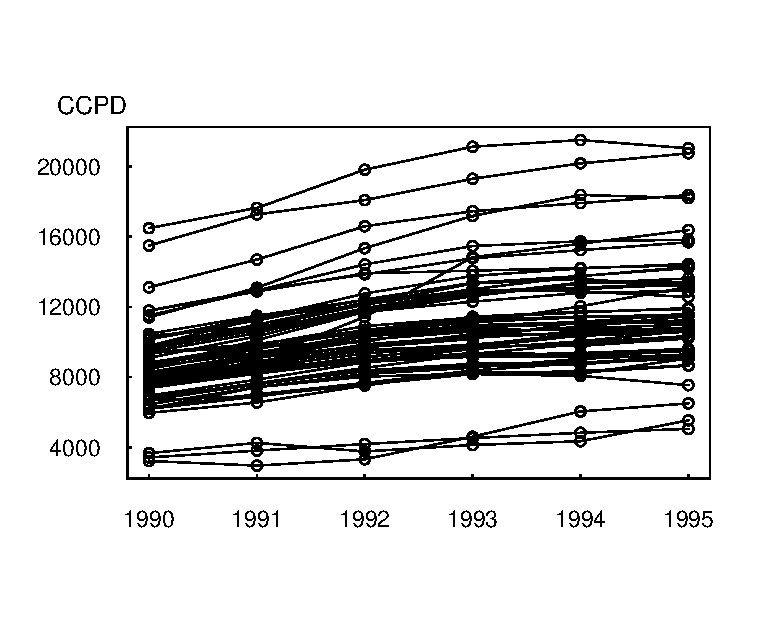
\includegraphics[width=.7\textwidth]
        {Chapter10LongData//F10MedicareTSPlot.eps}
    \caption{\label{F10:MedicareTSPlot} \small Multiple Time Series Plot of CCPD.
    Covered claims per discharge (CCPD) are plotted over $T=6$ years, 1990-1995.
    The line segments connect states; thus, we see that CCPD increases for almost every state over time.}
  \end{center}
\end{figure}



Figure \ref{F10:MedicarePlotWithLines} is a variation of a scatter
plot with symbols. This is a plot of CCPD versus number of
discharges. One could use different plotting symbols each state;
instead, we connect observations within a state over time. This plot
shows a positive overall relationship between CCPD and the number of
discharges. Like CCPD, we see a substantial state variation of
different numbers of discharges. Also like CCPD, the number of
discharges increases over time, so that, for each state, there is a
positive relationship between CCPD and number of discharges. The
slope is higher for those states with smaller number of discharges.
This plot also suggests that the number of discharges lagged by one
year is an important predictor of CCPD.

\begin{figure}[htp]
  \begin{center}
    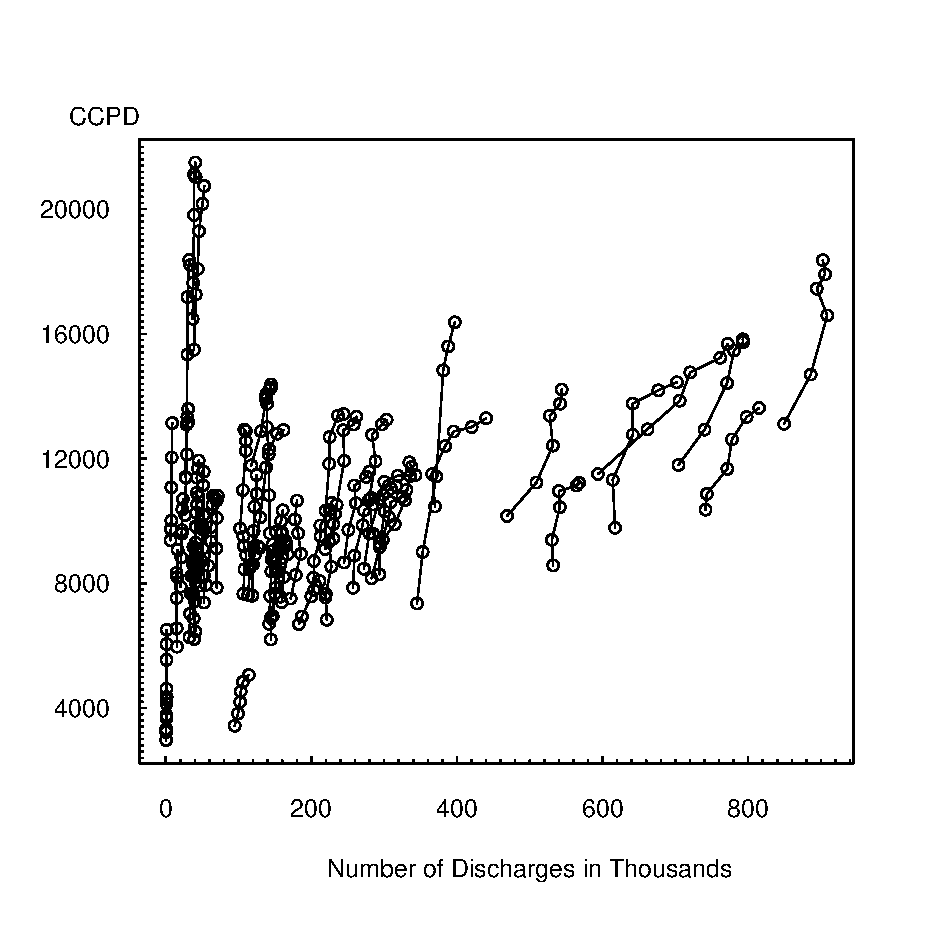
\includegraphics[width=.7\textwidth]
        {Chapter10LongData//F10MedicarePlotWithLines.eps}
    \caption{\label{F10:MedicarePlotWithLines} \small Scatter Plot of CCPD versus Number of Discharges.
    The line segments connect observations within a state over 1990-1995.
    We see a substantial state variation of numbers of discharges.
    There is a positive relationship between CCPD and number of discharges for each state.
    Slopes are higher for those states with smaller number of discharges.}
  \end{center}
\end{figure}


\subsubsection*{Trellis Plot}\index{plots!trellis}

A technique for graphical display that has recently become popular
in the statistical literature is a \emph{trellis plot}. This
graphical technique takes its name from a ``trellis'' which is a
structure of open latticework. When viewing a house or garden, one
typically thinks of a trellis as being used to support creeping
plants such as vines. We will use this lattice structure and refer
to a trellis plot as consisting of one or more panels arranged in a
rectangular array. Graphs that contain multiple versions of a basic
graphical form, each version portraying a variation of the basic
theme, promote comparisons and assessments of change. By repeating a
basic graphical form, we promote the process of communication.

Tufte (1997) states that using small multiples in graphical displays
achieves the same desirable effects as using parallel structure in
writing. Parallel structure in writing is successful because it
allows readers to identify a sentence relationship only once and
then focus on the meaning of each individual sentence element, such
as a word, phrase or clause. Parallel structure helps achieve
economy of expression and draw together related ideas for comparison
and contrast. Similarly, small multiples in graphs allow us to
visualize complex relationships across different groups and over
time. See Guideline Five in Section 21.3 for further discussion.

Figure \ref{F10:MedicareTrellisPlot} illustrates the use of small
multiples. In each panel, the plot portrayed is identical except
that it is based on a different state; this use of parallel
structure allows us to demonstrate the increasing covered claims per
discharge (CCPD) for each state. Moreover, by organizing the states
by average CCPD, we can see the overall level of CCPD for each state
as well as variations in the slope (rate of increase).

\begin{figure}[htp]
  \begin{center}
    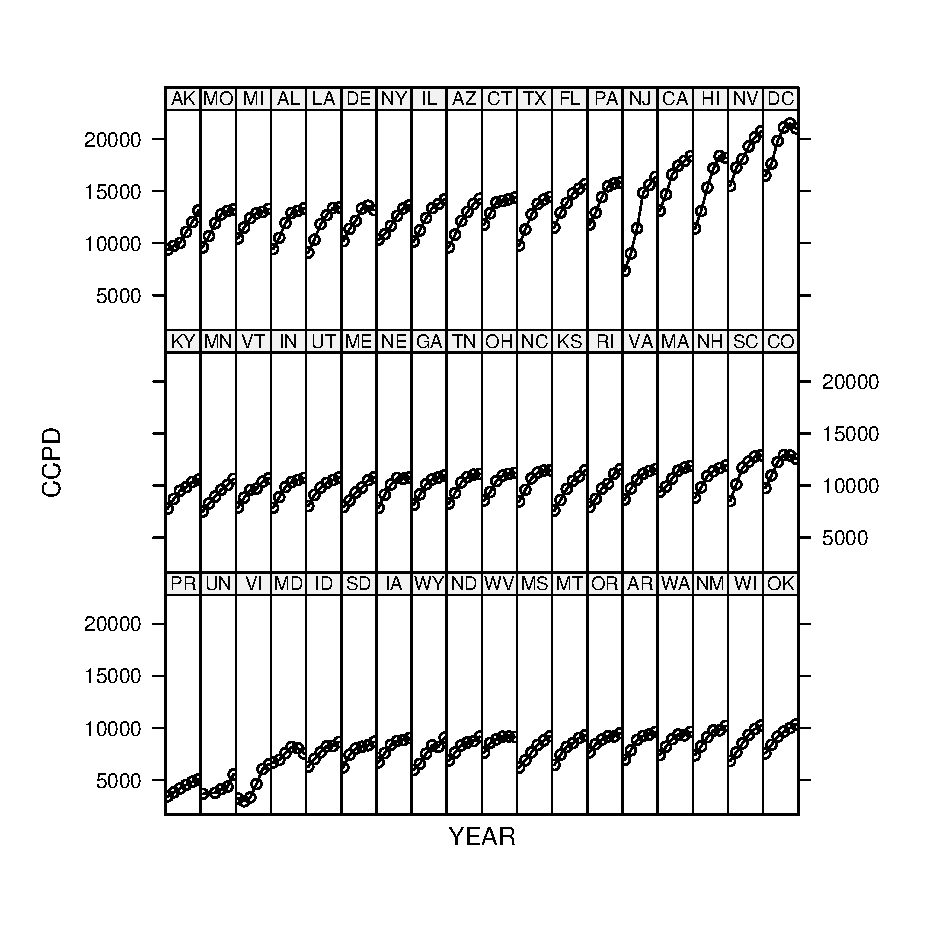
\includegraphics[width=.8\textwidth]
        {Chapter10LongData//F10MedicareTrellisPlot.eps}
    \caption{\label{F10:MedicareTrellisPlot} \small Trellis Plot of CCPD versus Year.
    Each of the 54 panels represents a plot of CCPD versus YEAR, 1990-1995 (the horizontal axis is suppressed).
    The increase for New Jersey (NJ) is unusually large.}
  \end{center}
\end{figure}


\linejed

\section{Basic Fixed Effects Models}\label{S10:FEModels}\index{time series models!longitudinal!basic fixed effects}

\subsubsection*{Data}

As described in Section \ref{S10:Intro}, we let $y_{it}$ denote the
dependent variable of the $i$th subject at the $t$th time point.
Associated with each dependent variable is a set of explanatory
variables. For the state hospital costs example, these explanatory
variables include the number of discharged patients and the average
hospital stay per discharge. In general, we assume there are $k$
explanatory variables $x_{it,1}, x_{it,2}, \ldots, x_{it,k}$ that
may vary by subject $i$ and time $t$. We achieve a more compact
notational form by expressing the $k$ explanatory variables as a $k
\times 1$ column vector
\begin{equation*}
\mathbf{x}_{it} = \left(\begin{array}{c}
  x_{it,1} \\
  x_{it,2} \\
  \vdots \\
 x_{it,k}
\end{array}\right) .
\end{equation*}

\noindent With this notation, the data for the $i$th subject
consists of:
\begin{equation*}
\left(\begin{array}{c}
  x_{i1,1},  x_{i1,2}, \ldots,  x_{i1,k}, y_{i1} \\
  \vdots \\
  x_{iT_i,1},  x_{iT_i,2}, \ldots,  x_{iT_i,k}, y_{iT_i} \\
\end{array}\right) = \left(\begin{array}{c}
  \mathbf{x}_{i1}^{\prime}, y_{i1} \\
  \vdots \\
  \mathbf{x}_{iT_i}^{\prime}, y_{iT_i} \\
\end{array}\right) .
\end{equation*}


\subsubsection*{Model}

A basic (and very useful) longitudinal data model is a special case
of the multiple linear regression model introduced in Section 3.2.
We use the modeling assumptions from Section 3.2.3 with the
regression function
\begin{eqnarray}\label{E10:BasicFEModel}
\mathrm{E}~y_{it} & = & \alpha_i + \beta_1 x_{it,1} + \beta_2
x_{it,2} + \cdots + \beta_k x_{it,k} \nonumber\\
& = & \alpha_i + \mathbf{x}_{it}^{\prime} \boldsymbol \beta,~~~~~~
t=1, \ldots, T_i,~~ i=1, \ldots, n .
\end{eqnarray}
This is the \textit{basic fixed effects model}.

The parameters $\{\beta_j\}$ are common to each subject and are
called \emph{global}, or \emph{population}, parameters. The
parameters $\{\alpha_i\}$ vary by subject and are known as
\textit{individual}, or \textit{subject-specific}, parameters. In
many applications, the population parameters capture broad
relationships of interest and hence are the parameters of interest.
The subject-specific parameters account for the different features
of subjects, not broad population patterns. Hence, they are often of
secondary interest and are called \emph{nuisance} parameters. In
Section \ref{S10:REModels}, we will discuss the case where
$\{\alpha_i\}$ are random variables. To distinguish from this case,
this section treats $\{\alpha_i\}$  as non-stochastic parameters
that are called ``fixed effects.''

The subject-specific parameters help to control for differences, or
``heterogeneity'' among subjects. The estimators of these parameters
use information in the repeated measurements on a subject.
Conversely, the parameters $\{\alpha_i\}$ are non-estimable in
cross-sectional regression models without repeated observations.
That is, with $T_i$ = 1, the model $y_{it}  =  \alpha_i + \beta_1
x_{it,1} + \beta_2 x_{it,2} + \cdots + \beta_k x_{it,k} +
\varepsilon_{it}$ has more parameters ($n+k$) than observations
($n$) and thus, we cannot identify all the parameters. Typically,
the disturbance term $\varepsilon_{it}$ includes the information in
$\alpha_i$ in cross-sectional regression models. An important
advantage of longitudinal data models when compared to
cross-sectional regression models is the ability to separate the
effects of  $\{\alpha_i\}$ from the disturbance terms
$\{\varepsilon_{it}\}$. By separating out subject-specific effects,
our estimates of the variability become more precise and we achieve
more accurate inferences.


\subsubsection*{Estimation}

Estimation of the basic fixed effects model follows directly from
the least squares methods. The key insight is that the heterogeneity
parameters $\{\alpha_i\}$ simply represent a \emph{factor}, that is,
a categorical variable that describes the unit of observation. With
this, least squares estimation follows directly with the details
given in Section 4.4 and the supporting appendices.

\marginparjed{The heterogeneity parameters $\{\alpha_i\}$ can be
represented by a \emph{factor}, that is, a categorical variable that
describes the unit of observation.}\index{time series
models!longitudinal!least squares dummy variable}

As described in Chapter 4, one can replace categorical variables
with an appropriate set of binary variables. For this reason, panel
data estimators are sometimes known as \emph{least squares dummy
variable model} estimators. However, as we have seen in Chapter 4,
be careful on the statistical routines. For some applications, the
number of subjects can easily run into the thousands. Creating this
many binary variables is computationally cumbersome. When you
identify a variable as categorical, statistical packages typically
use more computationally efficient recursive procedures (described
in Section 4.7.2).

\marginparjed{In the basic fixed effects model, coefficients
associated with time-constant variables cannot be estimated.}

The heterogeneity factor $\{ \alpha_i \}$ does not depend on time.
Because of this, it is easy to establish that regression
coefficients associated with time-constant variables cannot be
estimated using the basic fixed effects model. In other words,
time-constant variables are perfectly collinear with the
heterogeneity factor. Because of this limitation, analysts often
prefer to design their studies to use the competing random effects
model that we will describe in Section \ref{S10:REModels}.

\newpage

\linejed

\textbf{Example: Medicare Hospital Costs - Continued.} We compare
the fit of the basic fixed effects model to ordinary regression
models. Model 1 of Table \ref{T10:MedicareRegression} shows the fit
of an ordinary regression model using number of discharges
(NUM\_DCHG), YEAR and average hospital stay (AVE\_DAYS). Judging by
the large $t$-statistics, each variable is statistically
significant. The intercept term is not printed.

Figure \ref{F10:MedicareTrellisPlot} suggests that New Jersey has an
unusually large increase. Thus, an interaction term, YEARNJ, was
created that equals YEAR if the observation is from New Jersey and
zero otherwise. This variable is incorporated in Model 2 where it
does not appear to be significant.

Table \ref{T10:MedicareRegression} also shows the fit of a basic
fixed effects model with these explanatory variables. In the table,
the 54 subject-specific coefficients are not reported. In this
model, each variable is statistically significantly, including the
interaction term. Most striking is the improvement in the overall
fit. The residual standard deviation ($s$) decrease from 2,731 to
530 and the coefficient of determination ($R^2$) increased from 29\%
to 99.8\%.



\begin{table}[h]
\scalefont{0.9} \caption{\label{T10:MedicareRegression} \small
Coefficients and Summary Statistics from Three Models}
\begin{tabular}{lrrrrrr}
\hline
 &\multicolumn{2}{c}{Regression}&\multicolumn{2}{c}{Regression}&\multicolumn{2}{c}{Basic Fixed} \\
 &\multicolumn{2}{c}{Model 1} &\multicolumn{2}{c}{Model 2}
 &\multicolumn{2}{c}{Effects Model} \\
 & Coefficient & $t$-statistic &Coefficient & $t$-statistic &Coefficient & $t$-statistic
 \\
 \hline
  NUM\_DCHG &       4.70 &       6.49 &       4.66 &       6.44 &      10.75 &       4.18 \\
      YEAR &     744.15 &       7.96 &     733.27 &       7.79 &     710.88 &      26.51 \\
  AVE\_DAYS &     325.16 &       3.85 &     308.47 &       3.58 &     361.29 &       6.23 \\
      YEARNJ &            &            &     299.93 &       1.01 &   1,262.46 &       9.82 \\
      \hline
     $s$ &   \multicolumn{2}{c}{2,731.90} &  \multicolumn{2}{c}{2,731.78} &  \multicolumn{2}{c}{529.45}            \\
        $R^2$ (in percent) &  \multicolumn{2}{c}{28.6} &  \multicolumn{2}{c}{28.8} & \multicolumn{2}{c}{99.8}        \\
        $R_a^2$ (in percent) &  \multicolumn{2}{c}{27.9} &  \multicolumn{2}{c}{27.9} & \multicolumn{2}{c}{99.8}        \\
        \hline
\end{tabular}
\scalefont{1.1111}
\end{table}


\linejed

\section{Extended Fixed Effects Models}\label{S10:FEModels2}\index{time series models!longitudinal!extended fixed effects}

\subsubsection*{Analysis of Covariance Models}

In the basic fixed effects model, no special relationships between
subjects and time periods are assumed. By interchanging the roles of
``$i$'' and ``$t$'', we may consider the regression function
\begin{equation*}
\mathrm{E}~y_{it} = \lambda_t + \mathbf{x}_{it}^{\prime} \boldsymbol
\beta.
\end{equation*}\index{time series
models!longitudinal!one-way fixed effects} Both this regression
function and the one in equation (\ref{E10:BasicFEModel}) are based
on traditional one-way analysis of covariance models introduced in
Section 4.4. For this reason, the basic fixed effects model is also
called the \emph{one-way fixed effects model}. By using binary
(dummy) variables for the time dimension, we can incorporate
time-specific parameters into the population parameters. In this
way, it is straightforward to consider the regression function
\begin{equation*}
\mathrm{E}~y_{it} = \alpha_i + \lambda_t + \mathbf{x}_{it}^{\prime}
\boldsymbol \beta ,
\end{equation*}
known as the \emph{two-way fixed effects model}.\index{time series
models!longitudinal!two-way fixed effects}

\bigskip
\linejed

\textbf{Example: Urban Wages.} Glaeser and Mar\'{e} (2001)
investigated the effects of determinants on wages, with the goal of
understanding why workers in cities earn more than their non-urban
counterparts. They examined two-way fixed effects models using data
from the National Longitudinal Survey of Youth (NLSY); they also
used data from the Panel Study of Income Dynamics (PSID) to assess
the robustness of their results to another sample. For the NLSY
data, they examined $n = 5,405$ male heads of households over the
years 1983-1993, consisting of a total of $N = 40,194$ observations.
The dependent variable was logarithmic hourly wage. The primary
explanatory variable of interest was a three level categorical
variable that measures the city size in which workers reside. To
capture this variable, two binary (dummy) variables were used: (1) a
variable to indicate whether the worker resides in a large city
(with more than one-half million residents), a ``dense metropolitan
area,'' and (2) a variable to indicate whether the worker resides in
a metropolitan area that does not contain a large city, a
``non-dense metropolitan area.'' The reference level is
non-metropolitan area. Several other control variables were included
to capture effects of a worker's experience, occupation, education
and race. When including time dummy variables, there were $k = 30$
explanatory variables in the reported regressions.

\linejed

\subsubsection*{Variable Coefficients Models}

In the Medicare hospital costs example, we introduced an interaction
variable to represent the unusually high increases in New Jersey
costs. However, an examination of Figure
\ref{F10:MedicareTrellisPlot} suggests that many other states are
also ``unusual.'' Extending this line of thought, we might wish to
allow each state to have its own rate of increase, corresponding to
the increased hospital charges for that state. We could consider a
regression function of the form
\begin{equation}\label{E10:MedicareVSlope}
\mathrm{E}~CCPD_{it} = \alpha_i + \beta_1 (NUM\_DCHG)_{it} +
\beta_{2i} (YEAR)_{t} + \beta_3 (AVE\_DAYS)_{it} ,
\end{equation}
where the slope associated with YEAR is allowed to vary with state
``$i$.''

Extending this line of thought, we write the regression function for
a \emph{variable coefficients} fixed effects model as\index{time
series models!longitudinal!variable coefficients}
\begin{equation*}
\mathrm{E}~y_{it} =  \mathbf{x}_{it}^{\prime} \boldsymbol \beta_i.
\end{equation*}
With this notation, we may allow any or all of the variables to be
associated with subject-specific coefficients. For simplicity, the
subject-specific intercept is now included in the regression
coefficient vector $ \boldsymbol \beta_i$.

\linejed

\textbf{Example: Medicare Hospital Costs - Continued.} The
regression function in equation (\ref{E10:MedicareVSlope}) was fit
to the data. Not surprisingly, it resulted in excellent fit in the
sense that the coefficient of determination is $R^2 = 99.915 \% $
and the adjusted version is $R_a^2 = 99.987 \% $. However, compared
to the basic fixed effects model, there are an additional 52
parameters, a slope for each state (54 states to begin with, minus
one for the `population' term and minus one for New Jersey already
included). Are the extra terms helpful? One way of analyzing this is
through the general linear hypothesis test introduced in Section
4.2.2. In this context, the variable coefficients model represents
the ``full'' equation and the basic fixed effects model is our
``reduced'' equation. From equation (4.4), the test statistic is
\begin{equation*}
F-\textrm{ratio} = \frac {(0.99915 - 0.99809)/52}{(1-0.99915)/213} =
5.11 .
\end{equation*}
Comparing this to the $F$-distribution with $df_1 = 52$ and $df_2 =
213$, we see that the associated $p$-value is less than 0.0001,
indicating strong statistical significance. Thus, this is one
indication that the variable slope model is preferred when compared
to the basic fixed effects model.

\linejed


\subsubsection*{Models with Serial Correlation}

In longitudinal data, subjects are measured repeatedly over time.
For some applications, time trends represent a minor portion of the
overall variation. In these cases, one can adjust for their presence
by calculating standard errors of regression coefficients robustly,
similar to the Section 5.7.2 discussion. However, for other
applications, getting a good understanding of time trends is vital.
One such application that is important in actuarial science is
prediction; for example, recall the Section \ref{S10:Intro}
discussion of an actuary predicting insurance claims for a small
business.

We have seen in Chapters 7--9 some basic ways to incorporate time
trends, through linear trends in time (such as the YEAR term in the
Medicare hospital costs example) or using dummy variables in time
(another type of one-way fixed effects model). Another possibility
is to use a lagged dependent variable as a predictor. However, this
is known to have some unexpected negative consequences for the basic
fixed effects model (see for example the discussion in Hsiao, 2003,
Section 4.2 or Frees, 2004, Section 6.3).

Instead, it is customary to examine the serial correlation structure
of the disturbance term $ \varepsilon_{it} = y_{it} -
\mathrm{E}~y_{it}.$ For example, a common specification is to use an
autocorrelation of order one, $AR(1)$, structure, such as
\begin{equation*}
\varepsilon_{it} = \rho_{\varepsilon} \varepsilon_{i,t-1} +
\eta_{it},
\end{equation*}
where $\{ \eta_{it} \}$ is a set of disturbance random variables and
$\rho_{\varepsilon}$ is the autocorrelation parameter. In many
longitudinal datasets, the small number of time measurements ($T$)
would inhibit calculation of the correlation coefficient
$\rho_{\varepsilon}$ using traditional methods such as those
introduced in Chapter 8. However, with longitudinal data, we have
many replications ($n$) of these short times series; intuitively,
these replications provide the information needed to provide
reliable estimates of the autoregressive parameter.


\section{Random Effects Models}\label{S10:REModels}\index{time series models!longitudinal!random effects}


Suppose that you are interested in studying the behavior of subjects
that are randomly selected from a population. For example, you might
wish to predict insurance claims for a small business, using
characteristics of the business as well as past claims history.
Here, the set of small businesses may be randomly selected from a
larger database. In contrast, the Section \ref{S10:FEModels}
Medicare example dealt with a fixed set of subjects. That is, it is
difficult to think of the 54 states as a subset from some
``super-population'' of states. For both situations, it is natural
to use subject-specific parameters, $\{\alpha_i \}$, to represent
the heterogeneity among subjects. Unlike Section \ref{S10:FEModels},
we now discuss situations in which it is more reasonable to
represent $\{\alpha_i \}$ as random variables instead of fixed, yet
unknown, parameters. By arguing that $\{\alpha_i \}$ are draws from
a distribution, we will have the ability to make inferences about
subjects in a population that are not included in the sample.

\subsubsection*{Basic Random Effects Model}\index{time
series models!longitudinal!basic random effects}

The \emph{basic random effects} model equation is
\begin{equation}\label{E10:BasicREModel}
y_{it} = \alpha_i + \mathbf{x}_{it}^{\prime} \boldsymbol \beta +
\varepsilon_{it},~~~~~~ t=1, \ldots, T_i,~~ i=1, \ldots, n .
\end{equation}
This notation is similar to the basic fixed effects model. However,
now the term $\alpha_i$ is assumed to be a random variable, not a
fixed, unknown parameter. The term $\alpha_i$ is known as a
\emph{random effect}. \emph{Mixed effects} models are ones that
include random as well as fixed effects. Because equation
(\ref{E10:BasicREModel}) includes random effects ($\alpha_i$) and
fixed effects ($\mathbf{x}_{it}$), the basic random effects model is
a special case of the \emph{mixed linear model}. The general mixed
linear model is introduced in Section 15.1.

To complete the specification, we assume that $\{\alpha_i \}$  are
identically and independently distributed with mean zero and
variance $\sigma_{\alpha}^2$. Further, we assume that $\{\alpha_i
\}$ are independent of the disturbance random variables,
$\varepsilon_{it}$. Note that because E $\alpha_i$ = 0, it is
customary to include a constant within the vector $\mathbf{x}_{it}$.
This was not true of the fixed effects models in Section
\ref{S10:FEModels} where we did not center the subject-specific
terms about 0.

Linear combinations of the form $\mathbf{x}_{it}^{\prime}
\boldsymbol \beta $ quantify the effect of known variables that may
affect the dependent variable. Additional variables, that are either
unimportant or unobservable, comprise the ``error term.'' In
equation (\ref{E10:BasicREModel}), we may think of a regression
model $y_{it} = \mathbf{x}_{it}^{\prime} \boldsymbol \beta +
\eta_{it},$ where the error term $\eta_{it}$ is decomposed into two
components so that $\eta_{it}= \alpha_i + \varepsilon_{it}$. The
term $\alpha_i$ represents the time-constant portion whereas
$\varepsilon_{it}$ represents the remaining portion. To identify the
model parameters, we assume that the two terms are independent. In
the econometrics literature, this is known as the \emph{error
components} model; in the biological sciences, is is known as the
\emph{random intercepts} model.

\subsubsection*{Estimation}

Estimation of the random effects model does not follows directly
from least squares as with the fixed effects models. This is because
the observations are no longer independent due to the random effects
terms. Instead, an extension of least squares known as
\emph{generalized least squares} is used to account for this
dependency. Generalized least squares, often denoted by the acronym
\emph{GLS}, is a type of weighted least squares. Because random
effects models are special cases of mixed linear models, we will
introduce GLS estimation in this broader framework in Section 15.1.

To see the dependency among observations, consider the covariance
between the first two observations of the $i$th subject. Basic
calculations show

\begin{eqnarray*}
\mathrm{Cov}(y_{i1}, y_{i2}) &= &\mathrm{Cov}(\alpha_i +
\mathbf{x}_{i1}^{\prime} \boldsymbol \beta + \varepsilon_{i1},
\alpha_i + \mathbf{x}_{i2}^{\prime} \boldsymbol \beta +
\varepsilon_{i2}) \\
&= &\mathrm{Cov}(\alpha_i +\varepsilon_{i1}, \alpha_i +
 \varepsilon_{i2}) \\&= &\mathrm{Cov}(\alpha_i , \alpha_i)+\mathrm{Cov}(\alpha_i,
 \varepsilon_{i2})+\mathrm{Cov}(\varepsilon_{i1}, \alpha_i)+\mathrm{Cov}(\varepsilon_{i1},
 \varepsilon_{i2}) \\
 &= & \mathrm{Cov}(\alpha_i , \alpha_i) = \sigma^2_{\alpha} .
\end{eqnarray*}
The systematic terms $\mathbf{x}^{\prime} \boldsymbol \beta $ drop
out of the covariance calculation because they are non-random.
Further, the covariance terms involving $\varepsilon$ are zero
because of the assumed independence. This calculation shows that the
covariance between any two observations from the same subject is $
\sigma^2_{\alpha} $. Similar calculations show that the variance of
an observation is $\sigma^2_{\alpha} +\sigma^2_{\varepsilon}.$ Thus,
the correlation between observations within a subject is
$\sigma^2_{\alpha} / (\sigma^2_{\alpha} +\sigma^2_{\varepsilon})$.
This quantity is known as the \emph{intra-class correlation}, a
commonly reported measure of dependence in random effects studies.


\linejed

\textbf{Example: Group Term Life.} \ecaptionjed{Group Term Life}
Frees, Young and Luo (2001) analyzed claims data provided by an
insurer of credit unions. The data contains claims and exposure
information from 88 Florida credit unions for years 1993-1996. These
are ``life savings'' claims from a contract between the credit union
and their members that provides a death benefit based on the
member's savings deposited in the credit union. Actuaries typically
price life insurance coverage with knowledge of an insureds' age and
gender, as well as other explanatory variables such as occupation.
However, for these data from small groups, often only a minimal
amount of information is available to understand claims behavior.

Of the $88 \times 4=352$ potential observations, 27 were not
available because these credit unions had zero coverage in that year
(and thus excluded). Thus, these data were unbalanced. The dependent
variable is the annual total claims from the life savings contract,
in logarithmic units. The explanatory variables were annual
coverage, in logarithmic units, and YEAR, a time trend.

A fit of the basic random effects model showed that both year and
the annual coverage had positive and  strongly statistically
significant coefficients. That is, the typical amount of claims
increased over the period studied and claims increased as coverage
increased, other things being equal. There were strong credit union
effects, as well. For example, the estimated intra-class correlation
was 0.703, also suggesting strong dependence among observations.

\linejed

\subsubsection*{Extended Random Effects Models}\index{time
series models!longitudinal!extended random effects}

Just as with fixed effects, random effects models can be easily
extended to incorporated variable coefficients and serial
correlations. For example, Frees et al. (2001) considered the model
equation
\begin{equation}\label{E10:REExample}
y_{it} = \alpha_{1i} + \alpha_{2i} \mathrm{LNCoverage}_{it}+ \beta_1
+ \beta_2 \mathrm{YEAR}_t+ \beta_3 \mathrm{LNCoverage}_{it}+
\varepsilon_{it} ,
\end{equation}
where $\mathrm{LNCoverage}_{it}$ is the logarithmic life savings
coverage. As with the basic model, it is customary to use a mean
zero for the random effects. Thus, the overall intercept is
$\beta_1$ and $\alpha_{1i}$ represents credit union deviations.
Further, the overall or global slope associated with
$\mathrm{LNCoverage}$ is $\beta_3$ and $\alpha_{2i}$ represents
credit union deviations. Put another way, the slope corresponding to
$\mathrm{LNCoverage}$ for the $i$th credit is $\beta_3 +
\alpha_{2i}$.

More generally, the \emph{variable coefficients random effects
model} equation can be written as
\begin{equation}\label{E10:REModel}
y_{it} = \mathbf{x}_{it}^{\prime} \boldsymbol \beta +
\mathbf{z}_{it}^{\prime} \boldsymbol \alpha _i + \varepsilon_{it}.
\end{equation}
As with the fixed effects variable coefficients model, we may allow
any or all of the variables to be associated with subject-specific
coefficients. The convention used in the literature is to specific
fixed effects through the systematic component
$\mathbf{x}_{it}^{\prime} \boldsymbol \beta$ and random effects
through the component $\mathbf{z}_{it}^{\prime} \boldsymbol \alpha
_i$. Here, the vector $\mathbf{z}_{it}$ is typically equal to or a
subset of $\mathbf{x}_{it}$ although it need not be so. With this
notation, we now have a vector of random effects $\boldsymbol \alpha
_i$ that are subject-specific. To reduce to our basic model, one
only needs to choose $\boldsymbol \alpha _i$ to be a scalar (a $1
\times 1$ vector) and $\mathbf{z}_{it}\equiv 1.$ The example in
equation (\ref{E10:REExample}) results from choosing $\boldsymbol
\alpha _i = (\alpha_{1i}, \alpha_{2i})^{\prime}$ and
$\mathbf{z}_{it} = (1, \mathrm{LNCoverage}_{it})^{\prime}$.

As with fixed effects models, one can readily incorporate models of
serial correlation into random effects models by specifying a
correlations structure for $\varepsilon_{i1}, \ldots,
\varepsilon_{iT}$. This feature is readily available in statistical
packages and is described fully in the Section \ref{S10:References}
references.



\section{Further Reading and References}\label{S10:References}

Longitudinal and panel data models are widely used. To illustrate,
an index of business and economic journals, \textit{ABI/INFORM},
lists 685 articles in 2004 and 2005 that use panel data methods.
Another index of scientific journals, the \textit{ISI Web of
Science}, lists 1,137 articles in 2004 and 2005 that use
longitudinal data methods. A book-long introduction to longitudinal
and panel data that emphasizes business and social science
applications is Frees (2004). Diggle et al. (2002) provides an
introduction from a biomedical perspective. Hsiao (2003) provides a
classic introduction from an econometric perspective.

Actuaries are particularly interested in predictions resulting from
longitudinal data. These predictions can form the basis for updating
insurance prices. This topic is discussed in Chapter 18 on
credibility and bonus-malus factors.\index{actuarial \& financial
terms and concepts!credibility}



\bigskip

\textbf{Chapter References}

\begin{multicols}{2}

\scalefont{0.9}

Diggle, Peter J., Patrick Heagarty, Kung-Yee Liang and Scott L.
Zeger (2002). \textit{Analysis of Longitudinal Data, Second
Edition}. Oxford University Press, London.

Frees, Edward W. (2004). \textit{Longitudinal and Panel Data:
Analysis and Applications in the Social Sciences.} Cambridge
University Press, New York.

Frees, Edward W., Virginia R. Young and Yu Luo (2001). Case studies
using panel data models. \emph{North American Actuarial Journal} 5
(4), 24-42.

Glaeser, E. L. and D. C. Mar\'{e} (2001). Cities and skills.
\emph{Journal of Labor Economics} 19, 316-342.

Hsiao, Cheng (2003). \textit{ Analysis of Panel Data, Second
Edition}. Cambridge University Press, New York.

Tufte, Edward R. (1997). \emph{Visual Explanations}. Cheshire,
Conn.: Graphics Press.




\scalefont{1.1111}

\end{multicols}
